\documentclass[a4paper, 12pt]{article}

\usepackage[T1]{fontenc}
\usepackage[polish]{babel} 
\usepackage[utf8]{inputenc} 
\usepackage{indentfirst}
\let\lll\undefined
\usepackage{amssymb}
\usepackage{setspace}
\usepackage{fancyhdr}
\usepackage{graphicx} 

\pagestyle{fancy} 
\newcommand{\mainmatter}{\clearpage \cfoot{\thepage\ of \pageref{LastPage}}
\pagenumbering{arabic}}

\begin{document}
	\begin{titlepage}
		
		\begin{center}
    	\vspace{5cm}
    		\Large\textit{\textbf{SPECYFIKACJA FUNKCJONALNA 
    		\\''WireWorld'' DLA JĘZYKA PROGRAMOWANIA JAVA}}\\ 
		\vspace{5cm}
		\end{center} 


		
	\end{titlepage}
\newpage
\mainmatter
\setlength{\headheight}{15pt}
\doublespacing
\tableofcontents
\newpage

	\section{Opis Ogólny}
		\subsection{Nazwa programu} 
			\textbf{Nazwa programu:} \texttt{wireworld}
			
		\subsection{Poruszany problem}
		\hspace*{1cm} Zbudowanie programu ''WireWorld'' autorstwa Briana Silvermana w języku Java.\newline
			\hspace*{1cm} ''WireWorld'' składa się z czterech stanów komórek:
			
		\begin{enumerate}
			\item Pusta - czarny kolor.
			\item Głowa elektronu - niebieski kolor. 
			\item Ogon elektronu - czerwony kolor.
			\item Przewodnik - żółty kolor.
		\end{enumerate}					
		
			\hspace*{1cm} Zestaw zasad przy tworzeniu nowej generacji  jest następujący:

		\begin{itemize}
			\item komórka pozostaje Pusta, jeśli była Pusta.
			\item komórka staje się Ogonem elektronu, jeśli była Głową elektronu.
			\item komórka staje się Przewodnikiem, jeśli była Ogonem elektronu.
			\item komórka staje się Głową elektronu tylko wtedy, gdy dokładnie 1 lub 2 sąsiadujące komórki są Głowami Elektronu.
			\item Komórka staje się Przewodnikiem w każdym innym wypadku.
		\end{itemize}
		
			\hspace*{1cm} Są dwa rodzaje sąsiedztw Moore'a i von Neumanna. W sąsiedztwie Moore'a mamy 8 przylegających komórek (znajdujących się: na południu, na południowym-zachodzie, na zachodzie, na północnym-zachodzie, na północy, na północnym-wschodzie, na wschodzie i na południowym-wschodzie) oraz w sąsiedztwie von Neumanna 4 przylegających komórek (na południu, zachodzie, północy i wschodzie). \newline
			\hspace*{1cm} W ''WireWorld'' stosuje się sąsiedztwo Moore'a.
\newpage
	\section{Opis funkcjonalności}
			\hspace*{1cm} Funkcjonalnością programu ''WireWorld'' jest wyświetlanie animacji złożonej z kolejnych plansz podanego układu elektronicznego, oraz zapisanie aktualnego
stanu planszy do pliku, który może potem zostać wczytany, by kontynuować
pracę.
		\subsection{Możliwości programu}
			\hspace*{1cm} Program będzie zawierał następujące możliwości:
		
 		\begin{enumerate}
 			\item Odczytywanie pliku tekstowego TXT za pomocą \texttt{Upload} interfejsu graficznego (GUI).
 			\item Zapisywanie do plików tekstowych TXT za pomocą interfejsu graficznego (GUI).
 			\item Wystartowanie pliku wejściowego dla kolejnych generacji za pomocą przyciska \texttt{PLAY} (GUI).
 			\item Zatrzymanie działania programu za pomocą przyciska \texttt{STOP} (GUI).
 			\item Użytkownik ma możliwość zacząć wszystko od nowa za pomocą przyciska \texttt{New Game} (GUI).
 			\item Użytkownik ma możliwość regulować prędkość symulacji kolejnych generacji za pomocą pola \texttt{Guzika} (GUI).
 			\item Użytkownik ma możliwość regulować symulacji kolejnych generacji za pomocą przyciska \texttt{STEP} (GUI).
 			\item Użytkownik ma możliwość wprowadzić komórki do planszy w trybie \texttt{online}.
 			\item Obsługa różnych błędnych danych.
 		\end{enumerate}
 		
 		\subsection{Jak korzystać z programu?}
 			\hspace*{1cm} Program posiada interfejs graficzny (GUI). Z tego powodu użytkownik ma możliwość w łatwy sposób uruchomić program.
 			\newline
 			\hspace*{1cm} Lista postępowań do wywołania programu:
 		
 		 	\begin{enumerate}
 			\item Poprawna ścieżka do pliku z danymi opisującymi pierwszą generację. Program wczytuje format: \texttt{*.txt.}
 			\item Prędkość symulowanych generacji.
 			\end{enumerate}
 			
 		\subsection{Uruchomienie programu}
			\hspace*{1cm}\textbf{Przykład wywołania programu:}
			\newline Krok 1: Upload
			\newline Krok 2: Play
			\newline Krok 3: Save
\newpage
	\section{Format danych i struktura katalogów} 

		\subsection{Struktura katalogów}
			\hspace*{1cm} Program ''WireWorld'' będzie zawierała kilka katalogów, w katalogie głównym będzie plik wywołania programu. 
			\newline\hspace*{1cm} Podkatalog \texttt{''test''} będzie zawierał testy jednostkowe.
			\newline\hspace*{1cm} Podkatalog \texttt{''src''} będzie zawierał kolejne katalogi, w których znajduję się kod źródłowy:
			
			\begin{enumerate}
 			\item \texttt{''GUI''}
 			\item \texttt{''FileIO''}
 			\item \texttt{''WireWorld''}
 			\item \texttt{''Front''}
 			\end{enumerate}
 			
		\subsection{Dane wejściowe}
			\hspace*{1cm} Program ''WireWorld'' otrzymuje dane wejściowe. Plik tekstowy \texttt{*.txt} lub tryb online. Plik tekstowy składa się:\newline
			\textbf{Przykład:} 
			\begin{itemize}
			\item ElectronTail: 24, 6;
			\item Field: 24, 7;
			\item ElectronHead: 24, 8;
			\item ElectronTail: 24, 9;
			\item Field: 24, 10;
			\item ElectronHead: 24, 11;
			\item ElectronTail: 24, 12;
			\item Field: 24, 13;
			\end{itemize}
			
			\hspace*{1cm}\textbf{Tryb online składa sie:}
			
			\begin{itemize}
			\item kliknięcie \textbf{lewą} muszką \texttt{1 raz} - przewodnik (żółty kolor)  
			\item kliknięcie \textbf{lewą} muszką \texttt{2 razy} - usunięcie przewodnika (czarny kolor) 
			\item kliknięcie \textbf{prawą} muszką \texttt{1 raz} - ogon elektronu (czerwony kolor)
			\item kliknięcie \textbf{prawą} muszką \texttt{2 razy} - głowa elektronu (niebieski kolor)
			\end{itemize}
		
		\subsection{Wyjściowe}
			\hspace*{1cm}  W wyniku działania programu jest możliwość zapisywania za pomocą przyciska \texttt{Upload} do pliku tekstowego. Wynik będzie zapisany w postaci przykładu danych wejściowych.
\newpage
	\section{Scenariusz działania programu.}
		\subsection{Scenariusz ogólny}
			\hspace*{1cm} Główne kroki działania programu:
			
			\begin{itemize}
			\item uruchomienie
			\item sprawdzanie, żeby przewodnik nie wyszedł za przedziału planszy.
			\item wykonanie symulacji
			\item zakończenie działania programu
			\end{itemize}

		\subsection{Ekran programu}
			\hspace*{1cm} Program posiada interfejs graficzny (GUI).
			
			\begin{itemize}
			\item \texttt{Step} - lewy górny róg.
			\item \texttt{Guzik} - lewy górny róg po \texttt{Step}.
			\item \texttt{Play} - centrum po \texttt{Guzik}.
			\item \texttt{New Game} - prawy górny róg po \texttt{Play}.
			\item \texttt{Płansza} - centrum.
			\item \texttt{Save} - dolny centrum.
			\item \texttt{Upload} - dolny centrum po \texttt{Save}.
			\end{itemize}
			
			\hspace*{1cm} Poniżej jest przedstawiony rysunek ekranu działania programu:
			
			\begin{figure}
			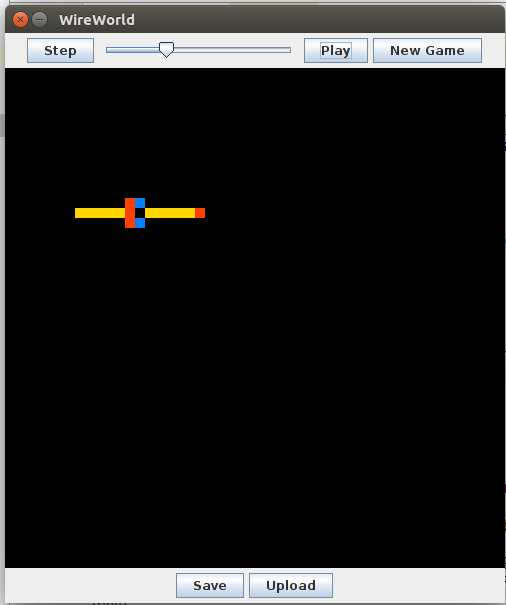
\includegraphics[width=\textwidth]{gui.png}
			\caption{ekran programu}
			\end{figure}	
		
	\section{Testowanie}
		\hspace{1cm} Do przetestowania kodu będzie używany kompilator \texttt{javac} razem z \texttt{Java Development Kit}. W programie będą prowadzone testy jednostkowe z wykorzystaniem biblioteki \texttt{AssertJ}, a GUI będzie przetestowany ręcznie podczas tworzenia aplikacji
\label{LastPage}~
\label{LastPageOfBackMatter}~		
\end{document}